%----------------------------------------------------------------------------------------
% Design del Sistema
%----------------------------------------------------------------------------------------

\documentclass[10pt]{softeng} % Document font size and equations flushed left

\usepackage{listings}

%----------------------------------------------------------------------------------------
%	DOCUMENT INFORMATION
%----------------------------------------------------------------------------------------

\include{current-phase}

\DocumentTitle{Design del Sistema} % Document title

\externaldocument[req:]{requirements}
\externaldocument[uc:]{use-case-model}
\externaldocument[sa:]{analisi-sistema}
\def\idVERSTOR{REQ\_VERSTOR\_F\_A\_1\,}
\def\shortidVERSTOR{REQ\_F\_1\,}

\def\idSECAUTH{REQ\_SECAUTH\_N\_A\_1\,}
\def\shortidSECAUTH{REQ\_N\_1\,}

\def\idCLIACC{REQ\_CLIACC\_F\_A\_2\,}
\def\shortidCLIACC{REQ\_F\_2\,}

\def\idAPPRCORR{REQ\_APPRCORR\_F\_A\_3\,}
\def\shortidAPPRCORR{REQ\_F\_3\,}

\def\idUSRBID{REQ\_USRBID\_F\_A\_4\,}
\def\shortidUSRBID{REQ\_F\_4\,}

\def\idLOGOP{REQ\_LOGOP\_N\_A\_2\,}
\def\shortidLOGOP{REQ\_N\_2\,}

\def\idCROPVEL{REQ\_CROPVEL\_F\_M\_5\,}
\def\shortidCROPVEL{REQ\_F\_5\,}

\def\idVERTIT{REQ\_VERTIT\_F\_M\_6\,}
\def\shortidVERTIT{REQ\_F\_6\,}

\def\idISCRCORR{REQ\_ISCRCORR\_F\_A\_7\,}
\def\shortidISCRCORR{REQ\_F\_7\,}

\def\idAPPBID{REQ\_APPBID\_F\_A\_8\,}
\def\shortidAPPBID{REQ\_F\_8\,}

\def\idDIPACC{REQ\_DIPACC\_F\_A\_9\,}
\def\shortidDIPACC{REQ\_F\_9\,}

\def\idCREABID{REQ\_CREABID\_F\_A\_10\,}
\def\shortidCREABID{REQ\_F\_10\,}

\def\idDISOPVEL{REQ\_DISOPVEL\_F\_M\_11\,}
\def\shortidDISOPVEL{REQ\_F\_11\,}

\def\idDISPAG{REQ\_DISPAG\_F\_A\_12\,}
\def\shortidDISPAG{REQ\_F\_12\,}

\def\idVERSAL{REQ\_VERSAL\_F\_A\_13\,}
\def\shortidVERSAL{REQ\_F\_13\,}

\def\idPRIVCORR{REQ\_PRIVCORR\_F\_A\_14\,}
\def\shortidPRIVCORR{REQ\_F\_14\,}


\def\iducCROPVEL{UC\_CROPVEL\_1\,}
\def\shortiducCROPVEL{UC\_1\,}
\def\iducDISPAG{UC\_DISPAG\_2\,}
\def\shortiducDISPAG{UC\_2\,}
\def\iducISCRCORR{UC\_ISCRCORR\_3\,}
\def\shortiducISCRCORR{UC\_3\,}
\def\iducBIDVIS{UC\_BIDVIS\_4\,}
\def\shortiducBIDVIS{UC\_4\,}
\def\iducDISOPVEL{UC\_DISOPVEL\_5\,}
\def\shortiducDISOPVEL{UC\_5\,}
\def\iducUSRBID{UC\_USRBID\_6\,}
\def\shortiducUSRBID{UC\_6\,}
\def\iducCREABID{UC\_CREABID\_7\,}
\def\shortiducCREABID{UC\_7\,}


%----------------------------------------------------------------------------------------

\begin{document}

\startofdocument{}


\begin{figure*}[h]
	\centering
	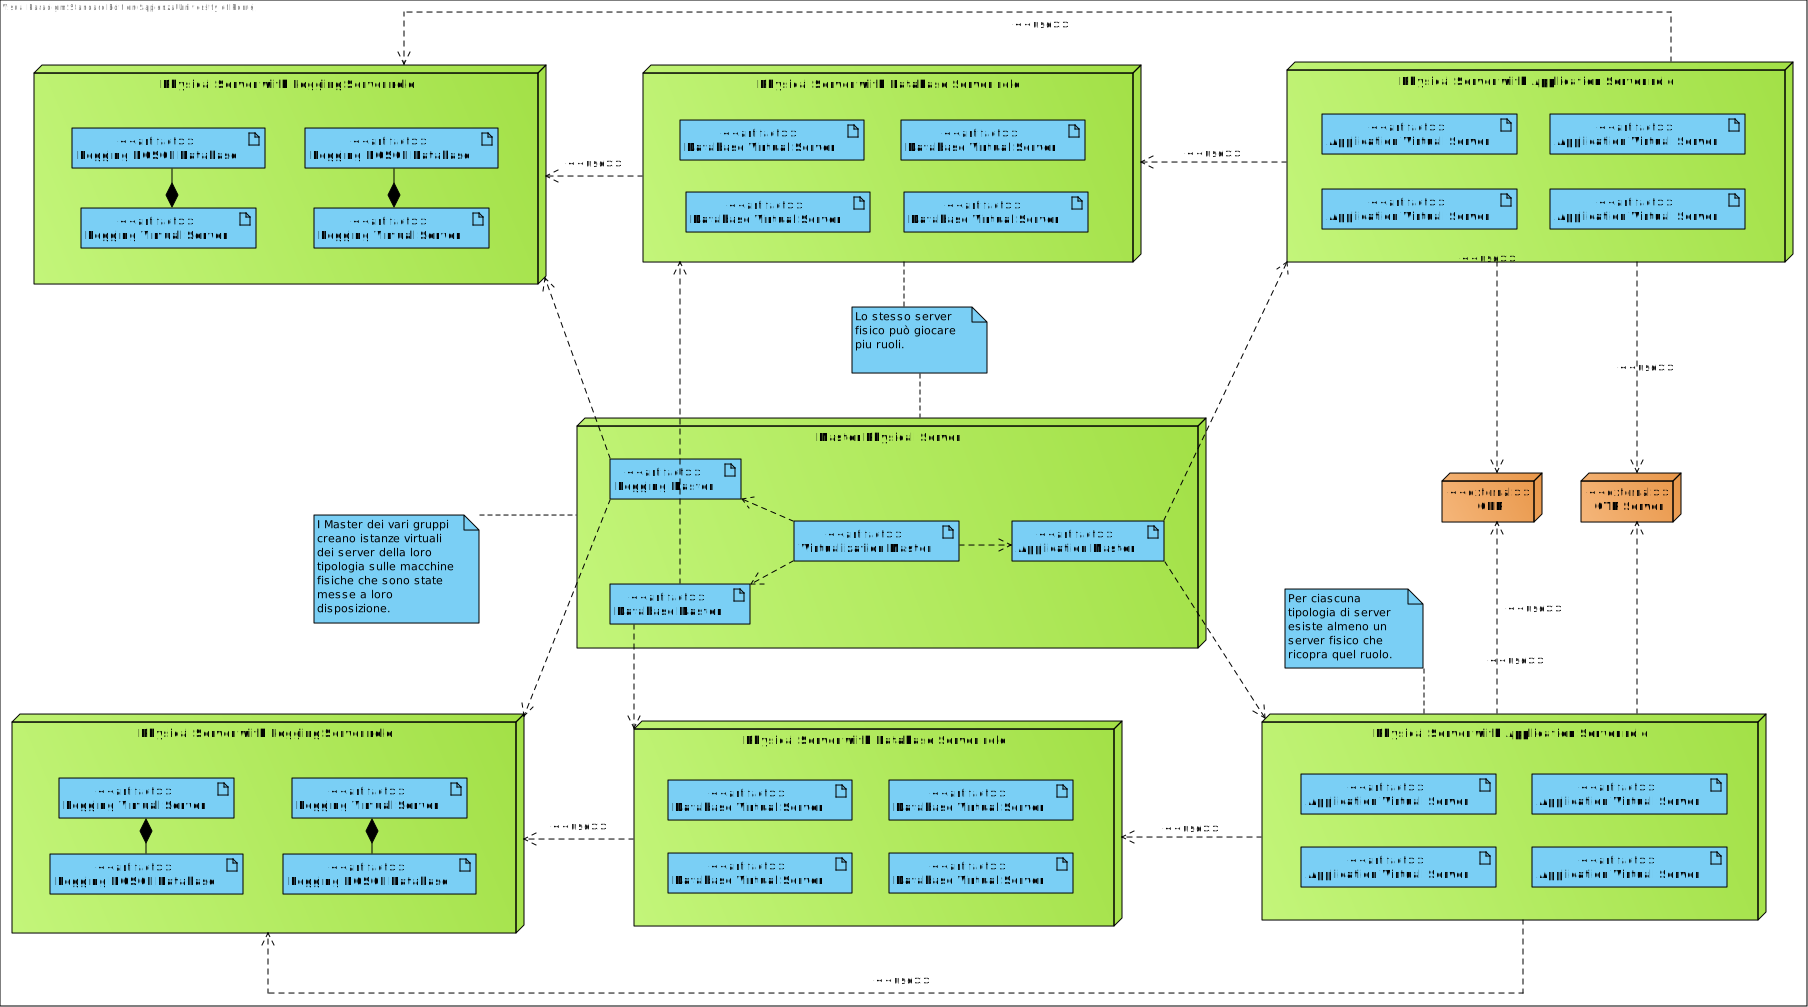
\includegraphics[width=\textheight, angle=90]{Images/Physical_View.eps}
	\caption{Diagramma di deployment del sistema.}
	\label{fig:physical-view}
\end{figure*}



\section{Classi di Design}

La realizzazione delle classi di design del sistema HBS \`e stata divisa in parti, separando:
\begin{enumerate}
	\item \label{itm:classi-fondamentali} classi principali, in particolare classi riguardanti:
		\begin{enumerate}
			\item gestione account utenti;
			\item gestione operazioni;
			\item comunicazione con OBP;
			\item verifica saldo e storico operazioni.
		\end{enumerate}
	\item classi secondarie, relative al sotto-sistema di operazioni veloci;
	\item classi relative al sotto-sistema di bidding;
	\item classi relative al sotto-sistema di Home Trading.
\end{enumerate}

Nella prima iterazione della fase di construction verranno approfondite le classi di cui al punto~\ref{itm:classi-fondamentali}.


\subsection{Classi Principali}

In figura~\ref{fig:classi-principali} sono illustrati i package e le classi principali del sistema di HBS, come definite sopra.

\begin{figure*}[h]
    \centering
    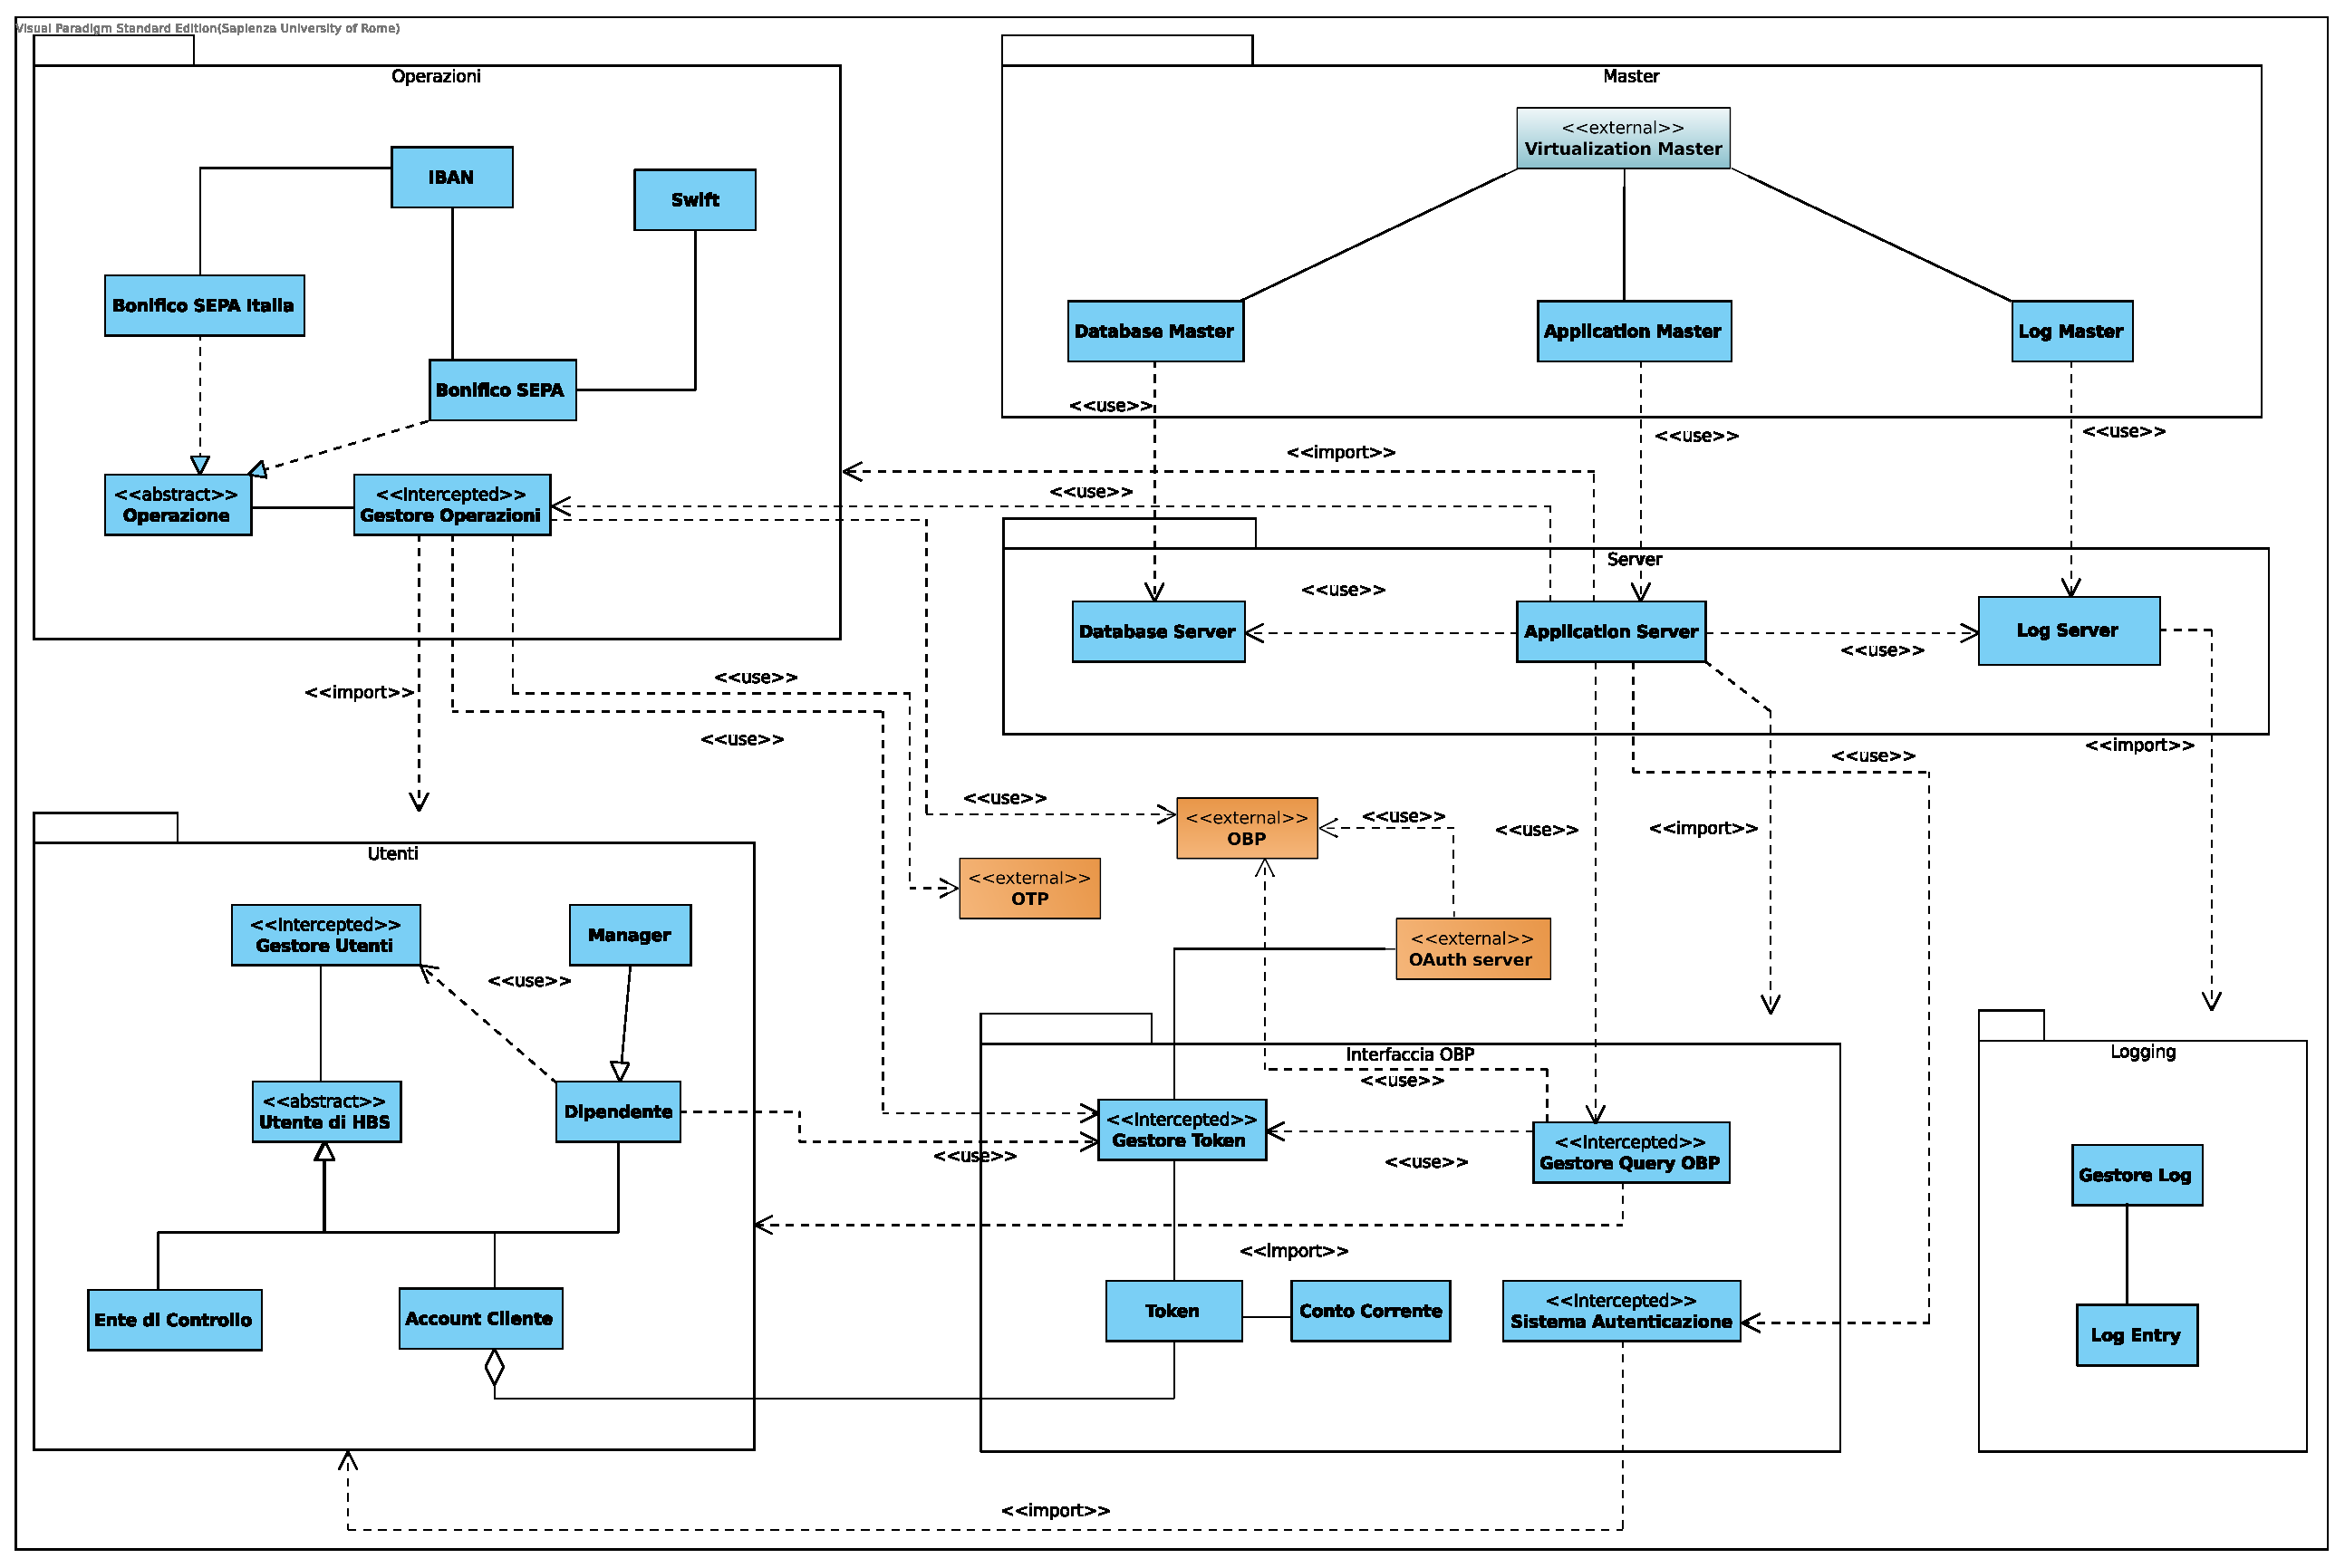
\includegraphics[width=\textheight, angle=90]{Images/Classi_Design.eps}
    \caption{Diagramma delle classi di design di HBS, ristretto alle classi principali.}
    \label{fig:classi-principali}
\end{figure*}

In figura~\ref{fig:classi-principali:operazioni} sono illustrate nel dettaglio le classi del package relativo alle operazioni.

\begin{figure*}[h]
    \centering
    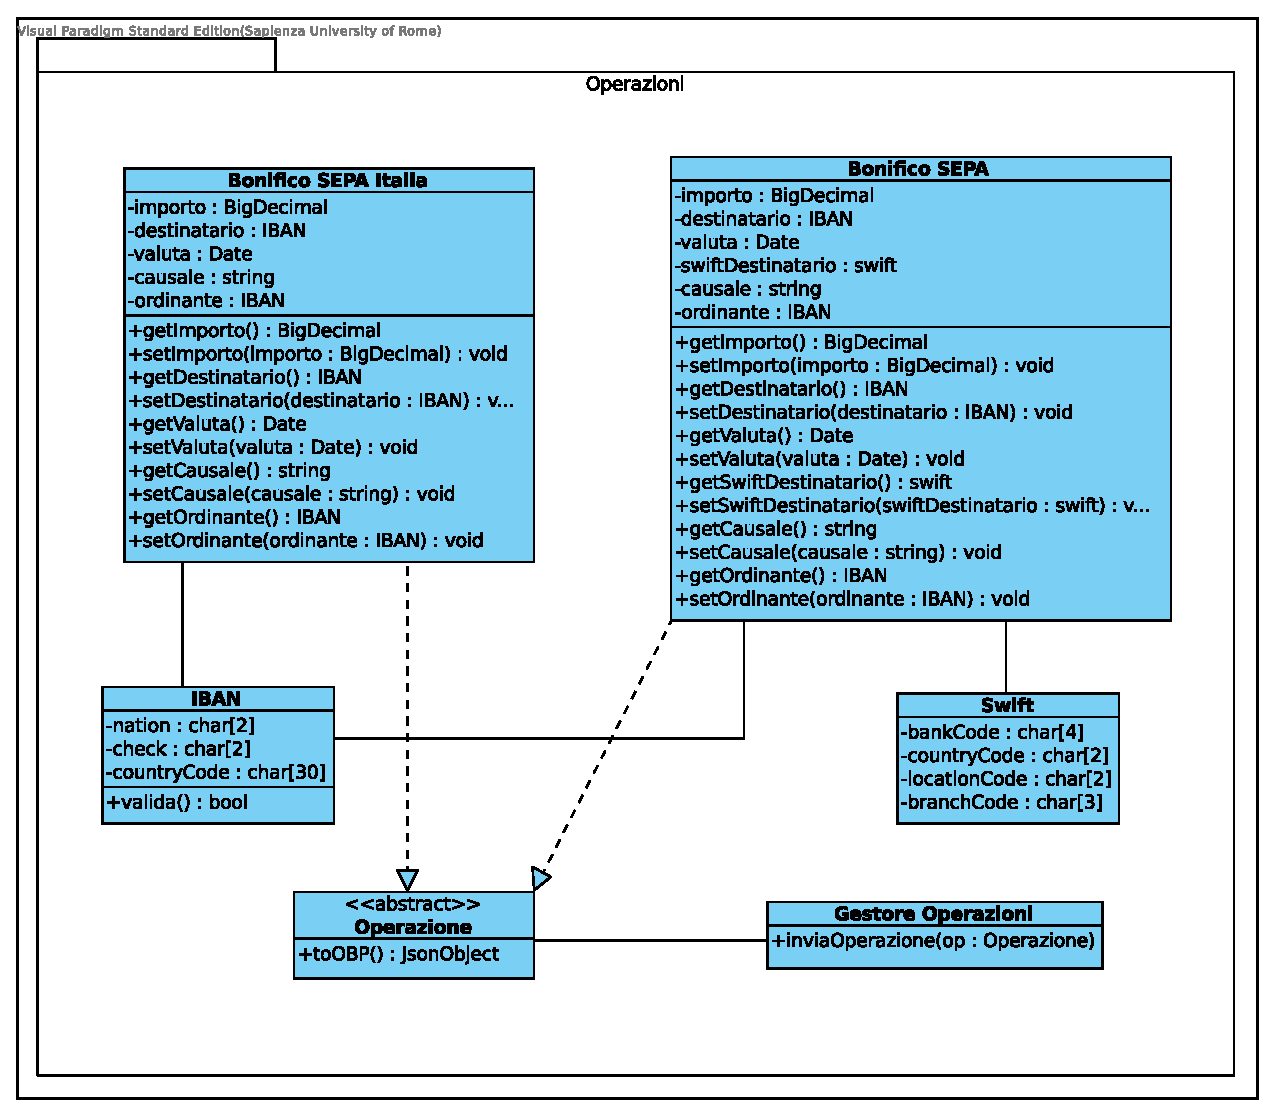
\includegraphics[width=\textwidth]{Images/Operazioni_Design.eps}
    \caption{Diagramma delle classi relative alle operazioni del sistema HBS.}
    \label{fig:classi-principali:operazioni}
\end{figure*}

In figura~\ref{fig:classi-principali:log} sono illustrate le classi del package relativo al sistema di logging.
Il sotto-sistema di logging utilizza il sistema di \emph{Class Interceptors} presente in Java EE 7.
Le annotazioni dei metodi sono riportate in figura come stereotipi.
Lo stereotipo \code{<<AroundInvoke>>} identifica l'annotazione \code{@AroundInvoke}.

I metodi delle classi soggette a logging sono decorati dallo stereotipo \code{Interceptors}, a cui corrisponde l'annotazione \code{@Interceptors(GestoreLog.class)}.
Le classi soggette a logging sono:
\begin{itemize}
	\item Gestore Operazioni;
	\item Gestore Query OBP;
	\item Gestore Token;
	\item Sistema Autenticazione.
\end{itemize}

\begin{figure*}[h]
    \centering
    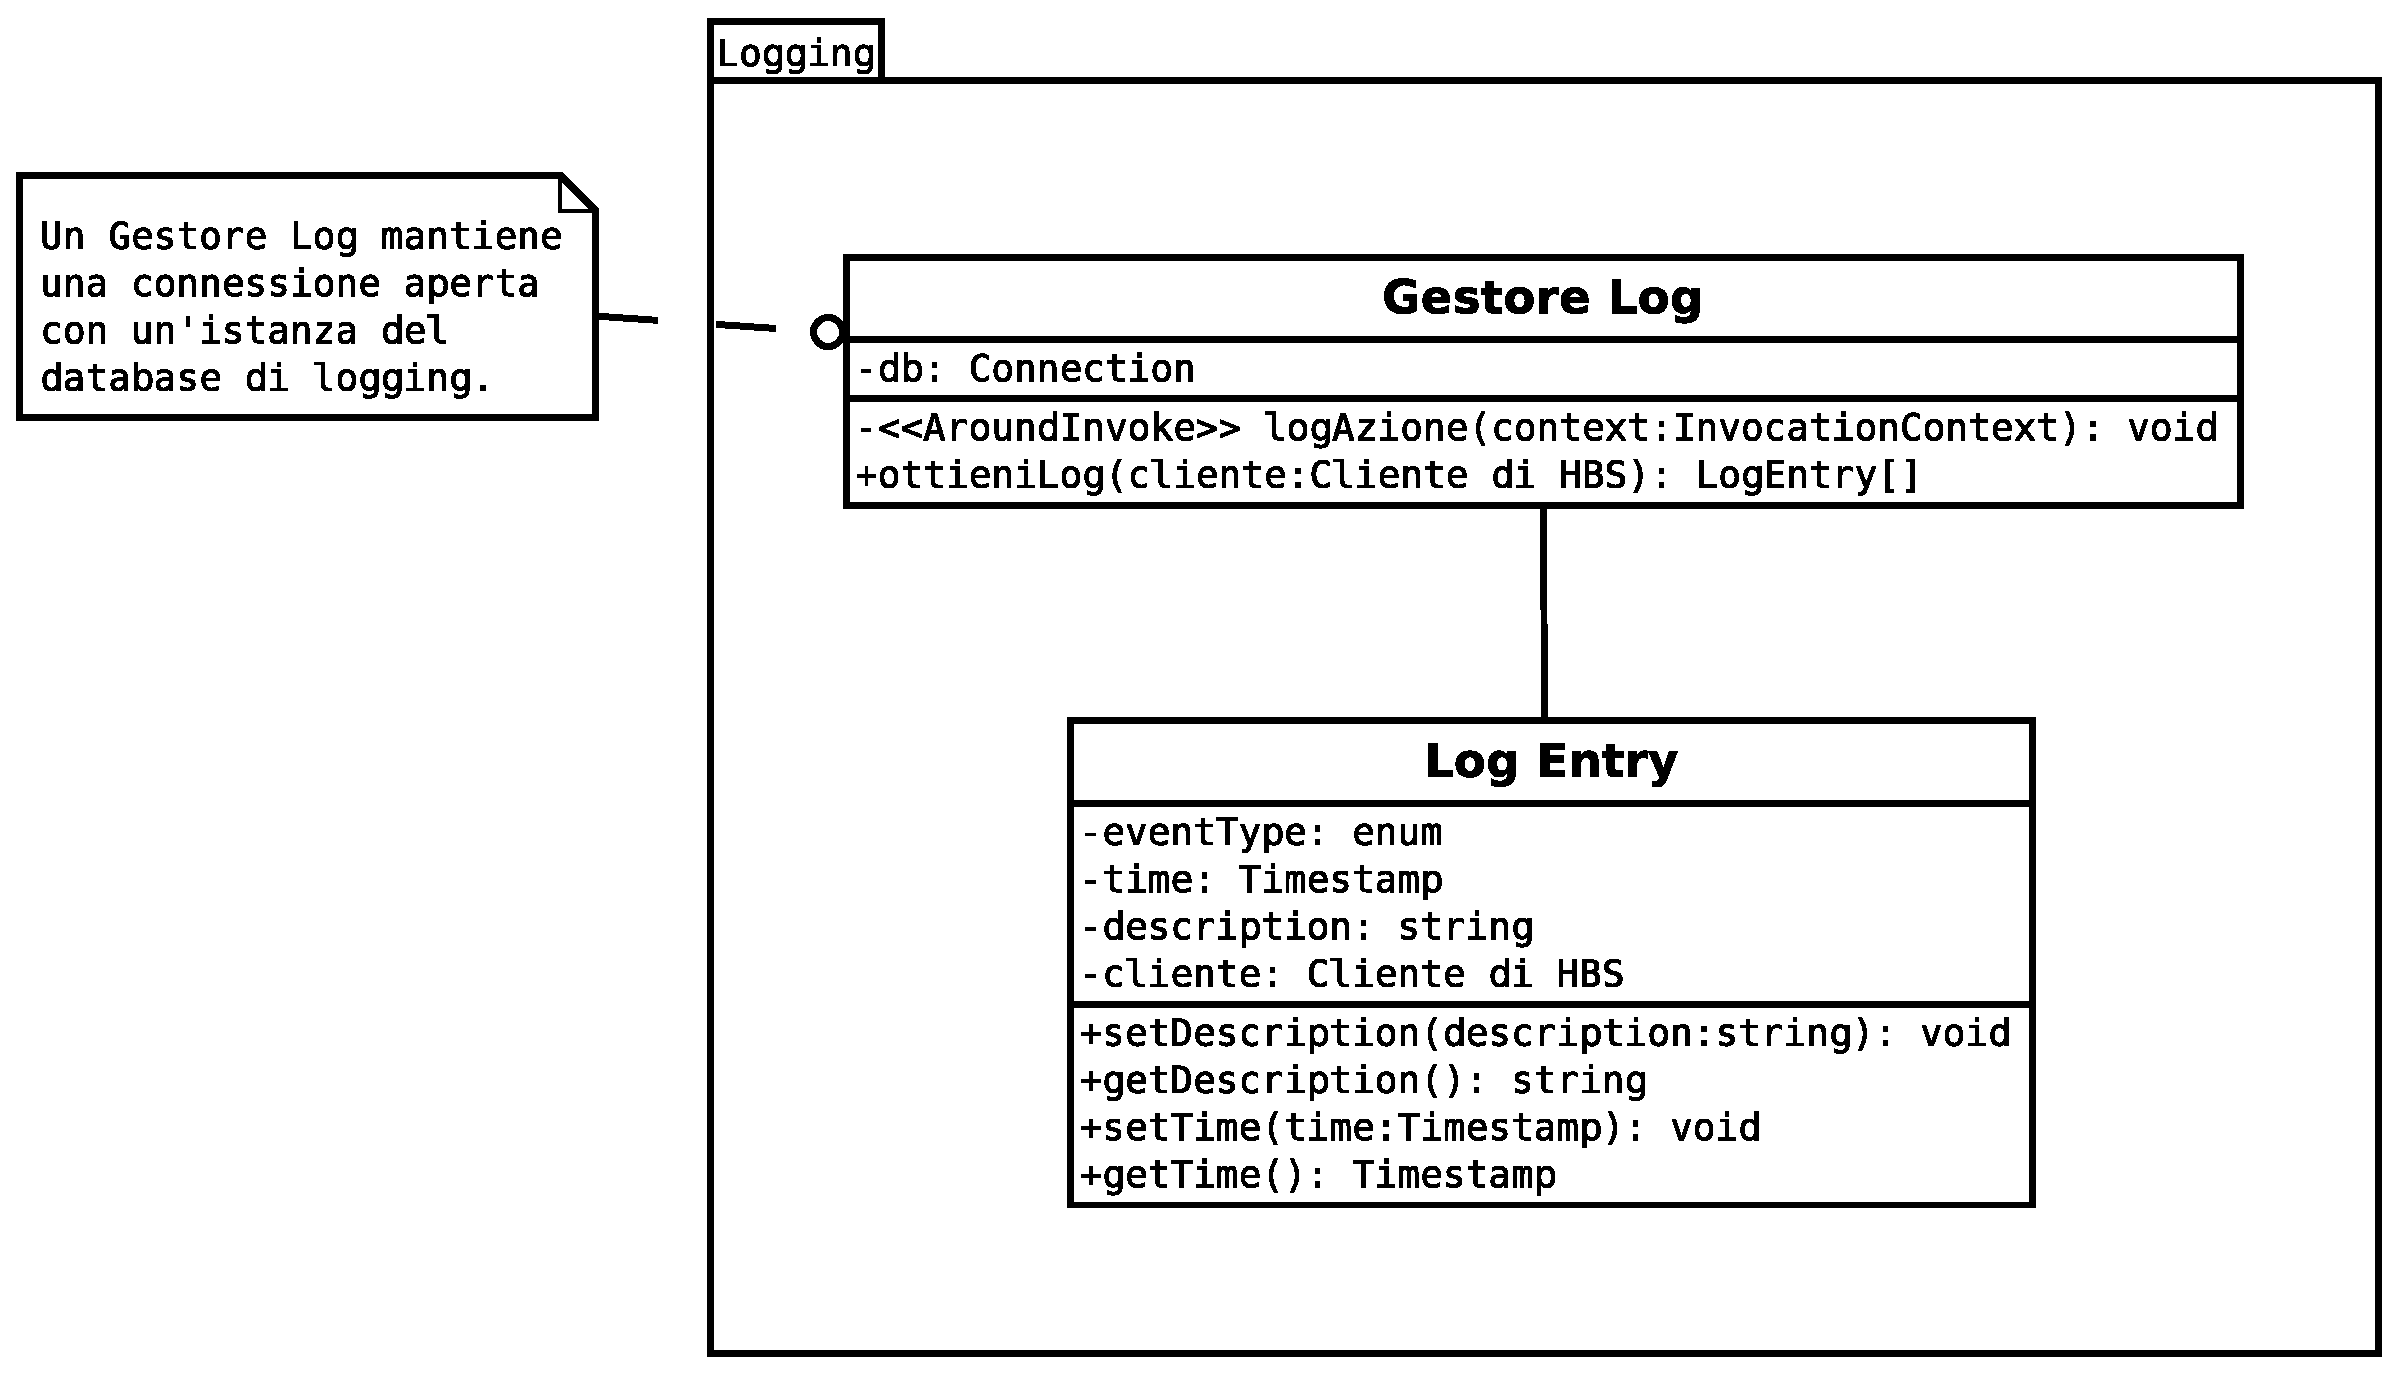
\includegraphics[width=\textwidth]{Images/dia/Logging.eps}
    \caption{Diagramma delle classi relative al sotto-sistema di Logging.}
    \label{fig:classi-principali:log}
\end{figure*}





\clearpage


\section{Interazione con OBP}

L'interfaccia di OBP è una interfaccia RESTful\footnote{L'interfaccia di OBP, in realtà, è in sola lettura. Estendiamo il suo funzionamento anche alla scrittura (inserimento di informazioni nel back-end), poiché l'estensione delle sue funzionalità in questo senso è, almeno logicamente, immediata.}, in cui i dati vengono trasmessi in formato json, e l'autenticazione è gestita tramite protocollo OAuth\cite{oauthrfc} (versione 1.0, prima revisione).

Il protocollo OAuth si basa sul modello client/server, e permette al client di accedere ad una risorsa protetta situata sul server e di propriet\`a di una terza entit\`a senza che questa (detta ``proprietario della risorsa'') debba condividere le proprie credenziali di accesso al server con il client.

In OBP i ruoli sono ripartiti nel seguente modo:
\begin{description}
	\item[Client] un'applicazione di terze parti che desideri accedere in lettura o in scrittura ai conti correnti presso la filiale (come il sistema HBS);
	\item[Server] l'API di OBP (e il back-end della banca soggiacente);
	\item[Resource owner] un correntista presso la banca iscritto a HBS;
	\item[Protected resource] un conto corrente di un correntista presso la banca;
	\item[Credentials] le credenziali di accesso alla banca del correntista;
	\item[Token] identificativo univoco fornito dal server al client.
\end{description}

Inserire un'operazione bancaria nel back-end della banca avviene con il seguente messaggio:
\begin{lstlisting}[basicstyle=\ttfamily]
POST /accounts/[ACCOUNT_ID]/transactions HTTP/1.1
[header]

{
    "this_account": {
        "id": [id account],
        "number": [numero conto],
        "IBAN": [iban conto],
        "swift_bic": [codice swift],
        "bank": {
            "national_identifier": [identificatore banca],
            "name": [nome banca]
        }
    },
    "other_account": {
        "holder": {
            "name": [nome beneficiario]
        },
        "number": [numero conto beneficiario],
        "IBAN": [iban beneficiario],
        "swift_bic": [codice swift],
        "bank": {
            "national_identifier": [identificatore istituto beneficiario],
            "name": [nome istituto beneficiario]
        },
    },
    "details": {
        "posted_by_user_id": [id utente],
        "posted_by_ip_address": [ip terminale],
        "type": "cash",
        "description": [causale],
        "posted": [data esecuzione],
        "value": {
            "currency": [valuta],
            "amount": [cifra]
        }
    }
}
\end{lstlisting}
Il messaggio di risposta contiene informazioni riguardo l'avvenuta presa in carico dell'operazione da parte del back-end della banca.



\section{Diagrammi di Sequenza}

Nei diagrammi di sequenza viene mostrata l'interazione fra le classi di design e i componenti del sistema per la realizzazione di un use case.

In figura~\ref{fig:sequenza:bonifico-sepa} viene illustrata la procedura per l'esecuzione di un bonifico SEPA da parte di un cliente di HBS.

\begin{figure*}[h]
    \centering
	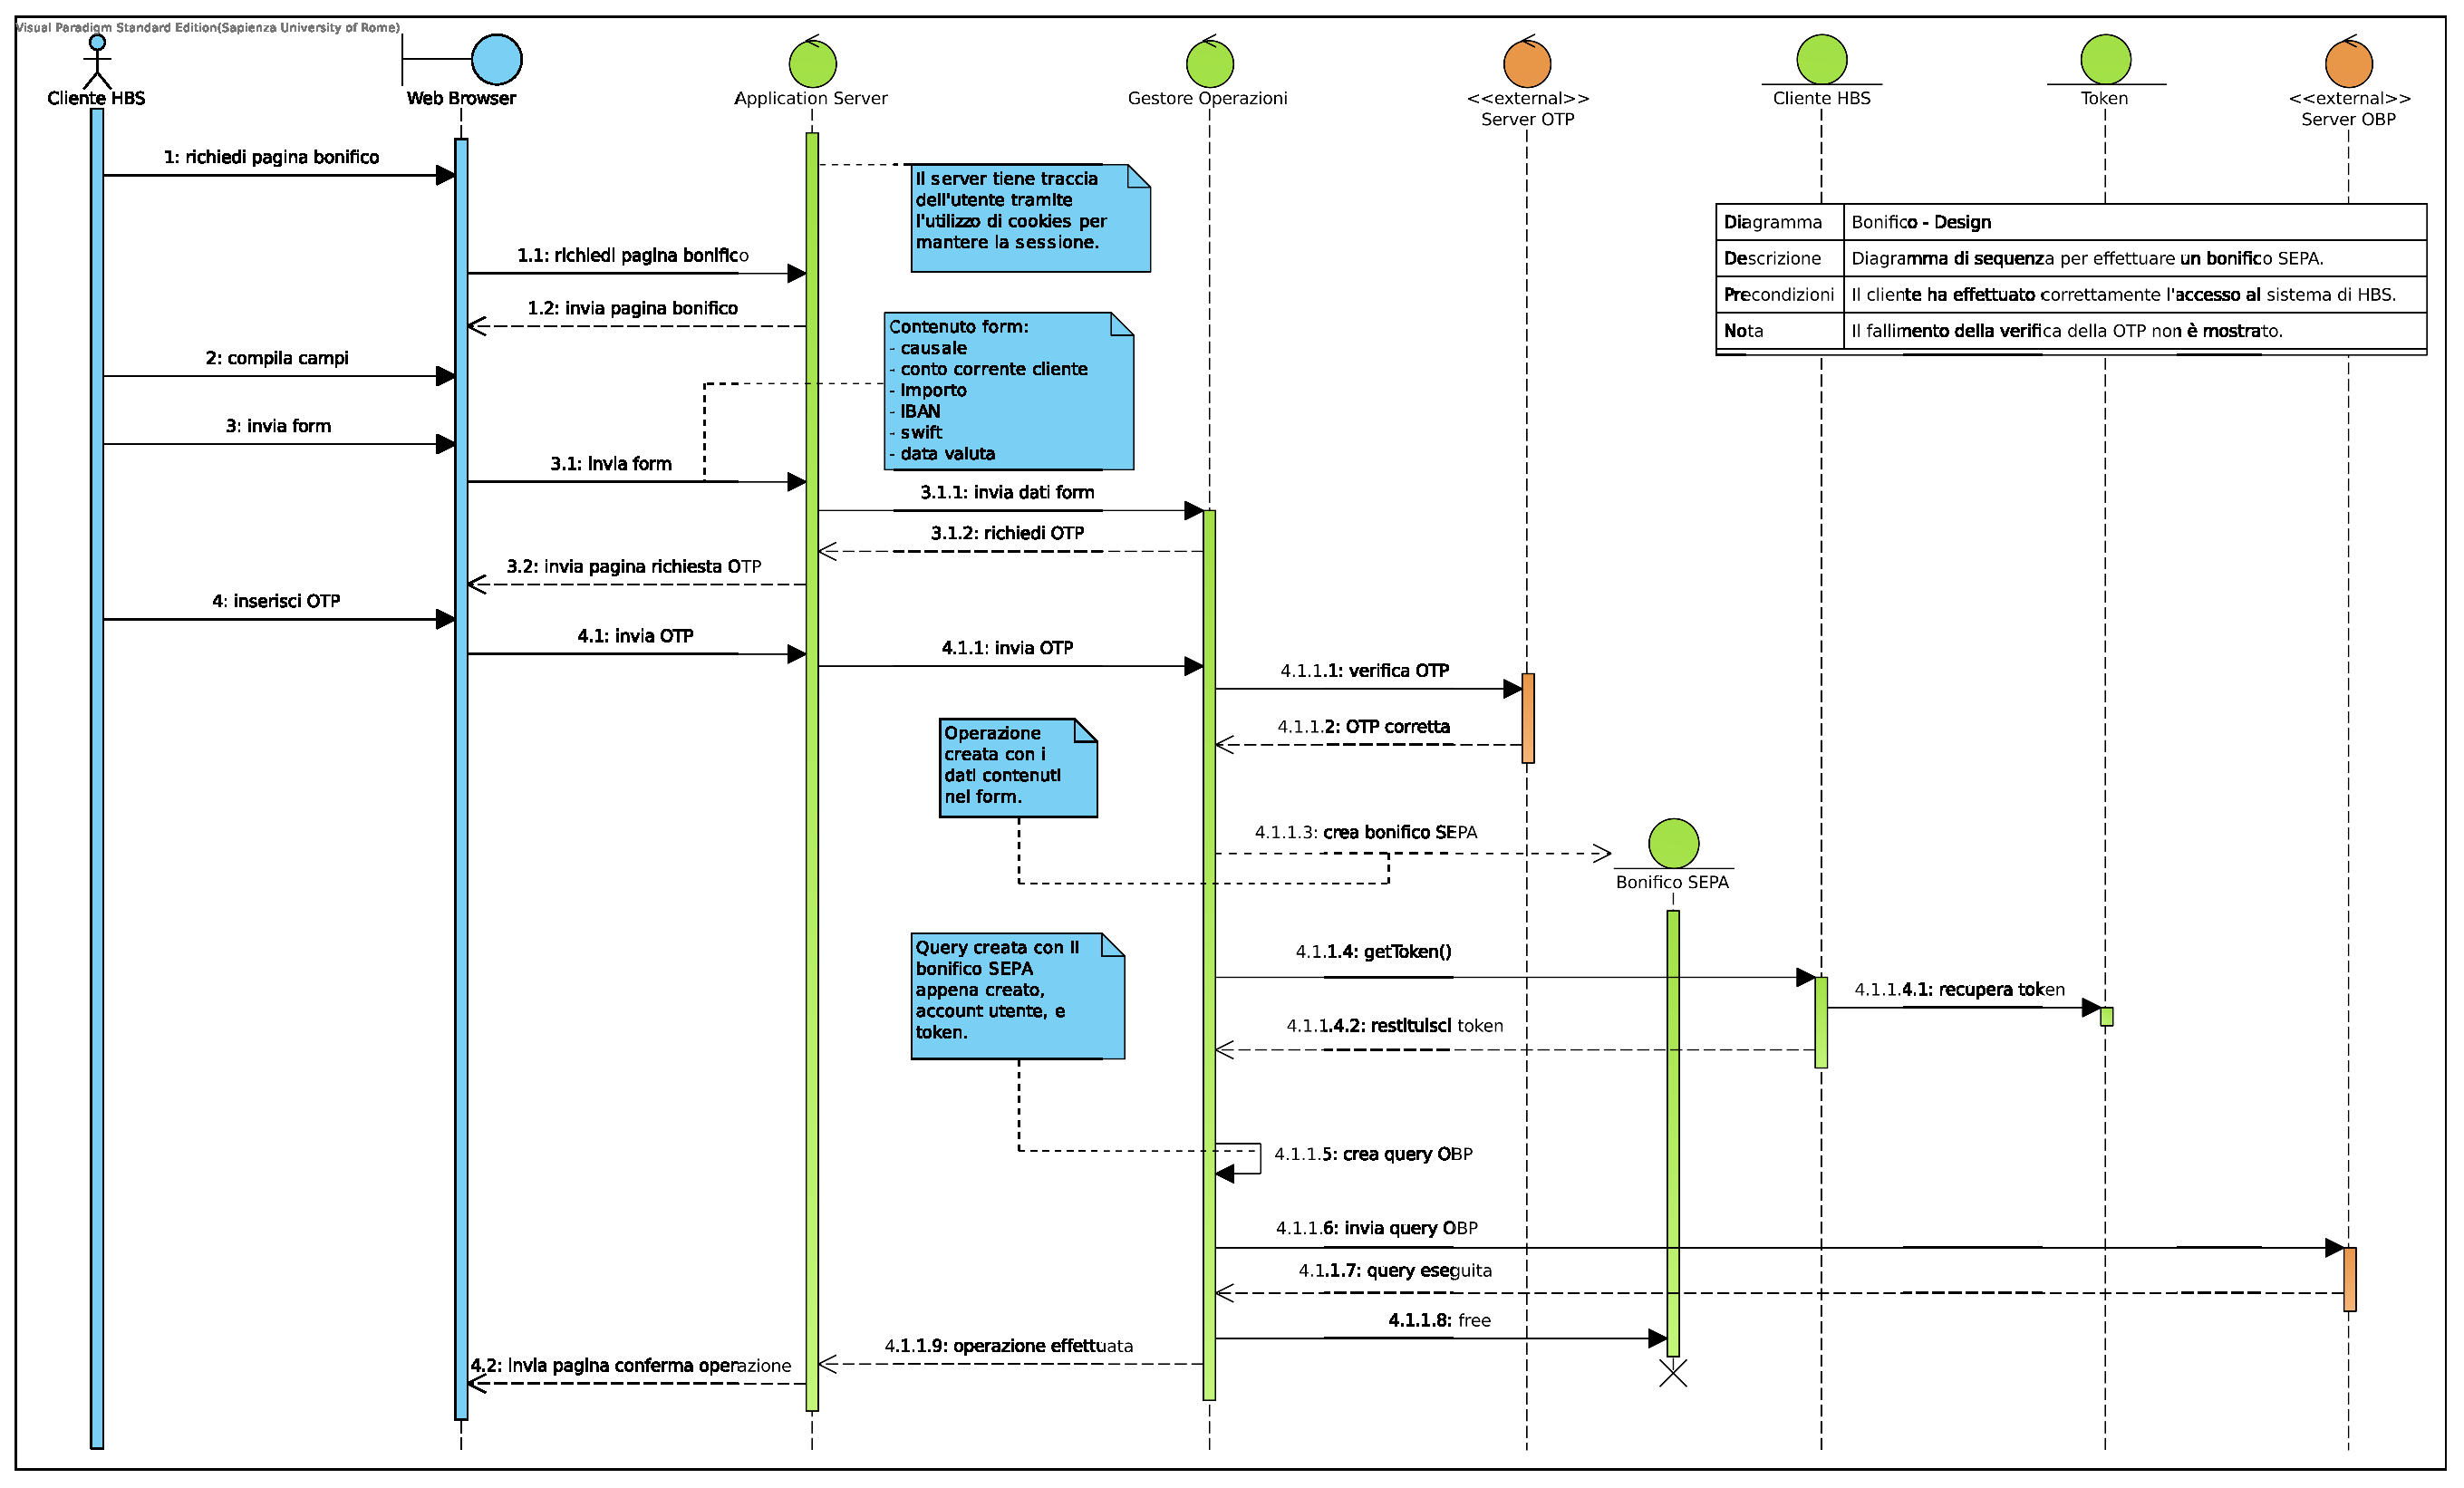
\includegraphics[width=\textheight, angle=90]{Images/Bonifico_-_Design.eps}
    \caption{Diagramma di sequenza relativo all'invio di un bonifico SEPA.}
    \label{fig:sequenza:bonifico-sepa}
\end{figure*}




\section{Registro modifiche}

\subsection{Construction}

\subsubsection{I iterazione}

Prima stesura documento.

\subsubsection{II iterazione}

Aggiunto diagramma classi sistema di logging.
Aggiornati diagrammi di sequenza per evidenziare ruolo logging.

%----------------------------------------------------------------------------------------
%	REFERENCE LIST
%----------------------------------------------------------------------------------------

%\nocite{banca_italia}
\printcustombib{}

%----------------------------------------------------------------------------------------
%	FIGURES
%----------------------------------------------------------------------------------------

\end{document}
